\documentclass[conference]{IEEEtran}

\usepackage[UTF8,scheme=plain,fontset=windows]{ctex}
\usepackage{cite}
\usepackage{amsmath,amssymb}
\usepackage{graphicx}
\usepackage{booktabs}
\usepackage{array}
\usepackage{url}

\renewcommand{\abstractname}{摘要}
\renewcommand{\IEEEkeywordsname}{关键词}
\renewcommand{\refname}{参考文献}

\title{面向版本化规范文档语义漂移的证据约束神经符号本体修复}

\author{\IEEEauthorblockN{匿名作者}
\IEEEauthorblockA{匿名单位\\
Email: anonymous@example.com}}

\begin{document}
\bstctlcite{IEEEexample:BSTcontrol}
\maketitle

\begin{abstract}
版本化规范文档会持续修订定义、义务、例外、作用域和生效条件。因此，基于早期文档版本构建的本体可能仍然保持逻辑一致，却包含已不再被当前证据语义支持的断言。本文提出 ECR-Repair，一种用于语义漂移下有限候选本体修复的证据约束神经符号框架。其核心设计是语义中间表示（Semantic Intermediate Representation, Semantic IR）：它作为自然语言规范证据与符号化 OWL/RDF 修复决策之间的神经符号接口。大语言模型用于解释证据，并在必要时验证候选蕴含关系；但候选内容在语义抽取阶段被隔离，从而避免将修复退化为“Evidence + Candidate $\rightarrow$ LLM $\rightarrow$ Answer”的直接提示。符号组件执行类型化语义归一化、约束感知候选排序、选择性门控，并通过 OWL 一致性、RDF 图差分检查和能力问题回归完成形式验证。在包含 264 个修复事件、1320 次运行和三类语义漂移模式的 RFC 基准上，ECR-Repair 达到 99.62\% 的闭包准确率和 99.24\% 的严格事件成功率，优于直接 LLM 基线和基础 Semantic IR 流水线。结果表明，面向演化规范来源的可靠本体修复不仅需要语言模型解释，还需要显式证据约束、候选内容隔离和形式符号闭包。
\end{abstract}

\begin{IEEEkeywords}
本体修复，语义漂移，神经符号推理，Semantic IR，大语言模型，OWL，RDF，证据 grounding
\end{IEEEkeywords}

\section{引言}

本体广泛用于表示法规要求、协议标准、领域政策和其他规范性知识。在这些场景中，正确性不仅取决于本体内部是否一致，还取决于其断言是否仍然被当前版本的规范文档支持。规范文档并非静态对象：新版本可能取代旧规范，例外条款可能覆盖一般规则，限定语可能改变多个陈述的作用域，生效日期也可能改变当前适用条件。这些变化会在本体与其证据来源之间造成语义漂移。

核心困难在于，语义漂移不同于语法错误或逻辑不一致。现有本体修复方法主要检测逻辑不一致，而语义过时但逻辑有效的断言仍然难以识别。一个过时断言可能格式良好、满足已声明词汇表，并通过推理机一致性检查。例如，断言某标准版本 $X$ 仍为当前版本，在版本 $Y$ 已取代 $X$ 后仍可能保持逻辑一致，因为如果本体没有显式表示并检查取代语义，就不会出现形式矛盾。因此，逻辑一致性 $\not\Rightarrow$ 语义正确性。单纯文本差分也不足够，因为版本化规范文档经常通过分散的时间锚点、例外条款和跨句作用域关系表达变化。

大语言模型（LLM）为解释这类规范语言提供了自然机制。然而，直接要求 LLM 修复本体会带来三个实际风险。第一，当证据不完整或语言结构复杂时，模型可能产生不受支持的幻觉式修复 \cite{ji2023hallucination}。第二，直接提示难以提供从证据到本体编辑的可追踪路径。第三，即使自然语言答案看似合理，也未必能产生保持图差分和下游能力问题行为的 OWL/RDF 补丁。这些限制在本体被用作规范约束的运行时表示时尤其突出。

本文提出 ECR-Repair，即一种证据约束神经符号本体修复框架。它不把修复视为直接生成，而是将任务分解为五个角色：
\[
\begin{gathered}
\text{规范证据}
\rightarrow
\text{Semantic IR}
\rightarrow
\text{符号决策}\\
\rightarrow
\text{回退验证}
\rightarrow
\text{OWL/RDF 验证}.
\end{gathered}
\]
语义中间表示（Semantic IR）是核心神经符号接口：它在候选排序之前将证据转换为类型化语义字段。例如，若旧本体声称规范 $X$ 是当前版本，而当前规范证据表明规范 $Y$ 更新 $X$ 并支配目标要求，则 Semantic IR 记录实体 $X$ 和 $Y$、更新关系、$Y$ 的当前或生效角色、$X$ 的过时或历史角色，以及支持证据片段。候选排序随后偏好以 $Y$ 替换 $X$ 的修复，并拒绝保留 $X$ 或反转更新方向的候选。

该流程显式分离证据解释和候选选择。语义解释模块不读取候选值、候选操作、候选标识符、候选分数或 top-$k$ 身份。只有在候选盲的 Semantic IR 固定之后，系统才暴露有限候选集。这避免了如下捷径：
\[
\text{Evidence + Candidate} \rightarrow \text{LLM} \rightarrow \text{Answer}
\]
并改为：
\[
\text{Evidence} \rightarrow \text{Semantic IR} \rightarrow \text{Candidate Ranking}.
\]
若排序仍然存在歧义，回退验证器可以独立评估候选，但只在候选感知的决策层中进行，并遵守固定的弃权规则。

本文会议版聚焦方法提出和初步实证验证。任务被定义为给定事件、证据窗口和有限候选集下的证据相对语义修复；自动漂移发现、开放语料检索和开放式候选生成不在本文范围内。

本文贡献如下：
\begin{itemize}
    \item 提出 ECR-Repair，一种面向版本化规范文档语义漂移的证据约束神经符号本体修复框架。
    \item 提出 Semantic IR 作为 LLM 证据解释与符号推理之间的显式接口，并给出候选内容隔离协议以防止排序前的候选泄漏。
    \item 定义已选 OWL/RDF 修复的形式闭包验证，并在 264 个 RFC 修复事件和 1320 次运行上评估该方法，显示其相较直接 LLM 和基础 Semantic IR 基线具有明显提升。
\end{itemize}

\section{相关工作}

\subsection{本体演化与修复}

本体演化和修复研究如何在保持可用性、一致性和约束满足的同时，将知识来源或概念化变化传播到本体中。近期 SHACL 和约束修复工作提供了一类场景：在显式 shape 约束下检测并修复 RDF 图违规 \cite{ahmetaj2022shacl,ahmetaj2025shacl}。这些方法对结构和逻辑质量至关重要，但它们本身不能保证断言仍被修订后的规范文档支持。

本文设置更窄且不同。我们假设潜在局部修复事件已被识别，并且有限可执行候选集已经给定。任务是选择其语义被当前证据支持的候选，并验证所得 OWL/RDF 补丁。这使语义解释位于形式闭包之前：形式检查能够拒绝格式错误、不一致或未声明的编辑，但不能判断一个形式有效候选是否最受当前规范证据支持。

\subsection{基于 LLM 的本体工程}

近期研究探索了 LLM 在本体学习、需求获取、能力问题生成、本体草拟和本体测试中的作用 \cite{giglou2024llms4ol,lippolis2025ontologygeneration,zhang2025ontochat,fathallah2025neongpt}。LLM 能降低从文本需求到结构化知识的成本，关于 LLM 与知识图谱的研究也显示了语言模型与符号图表示结合的广泛机会 \cite{pan2024llmkg}。与此同时，LLM 输出可能出现幻觉、结构不稳定或难以验证 \cite{ji2023hallucination}。

因此，ECR-Repair 对 LLM 采取保守用法。模型不直接重写本体，而是先将证据解释为 Semantic IR，再由后续符号决策层将该 IR 映射到候选编辑。当候选歧义仍然存在时，基于 LLM 的验证被用作回退蕴含检查，而不是无约束修复生成器。

\subsection{神经符号推理}

神经符号 AI 结合了神经模型的模式识别和语言理解能力，以及符号系统的显式结构、约束和推理能力 \cite{yu2023neurosymbolic}。知识图谱为这种集成提供了自然的符号载体，因为它以机器可检查形式编码实体、关系、约束和图结构 \cite{hogan2021knowledgegraphs}。检索增强生成进一步表明，当生成过程受检索或选择证据约束时，语言模型能够受益于外部证据 \cite{gao2024rag,asai2023selfrag}。

ECR-Repair 沿袭这一方向，但将其应用于版本化规范证据下的本体修复。神经层将证据转换为结构化语义表示；符号层执行类型约束、候选可接受性、图差分一致性和能力问题回归。当证据或排序信号不足时，系统应选择弃权而不是强行修复，这一点也受到选择性预测思想启发 \cite{gu2023selective}。

\section{问题形式化}

设 $O$ 为源本体，其中可能包含不再被当前规范证据支持的断言。设 $D$ 为一组版本化规范文档，$C=\{c_1,\ldots,c_k\}$ 为某局部修复事件的有限候选集。每个候选 $c_i$ 包含显示值和形式 OWL/RDF 编辑操作。输出为一个被选修复候选 $c^\ast$，或 \textsc{Abstain}。

输入为：
\[
(O,D,C),
\]
其中事件元数据指定目标 subject、predicate、语义类型和证据窗口。输出为：
\[
c^\ast \in C \cup \{\textsc{Abstain}\}.
\]
一个候选只有在被当前证据支持且其 OWL/RDF 补丁通过形式验证时才会被接受。仅用于评估的私有 oracle 被排除在所有模型提示和决策输入之外。

本文研究证据相对语义修复，而不是自动漂移发现。任务假设潜在漂移位置、相关证据窗口和有限候选集已被提供。因此，本文方法不是一个扫描完整语料、检索全部证据、生成候选补丁或证明所有文档版本间历史漂移的端到端系统。

这一区分很重要，因为语义漂移是相对于证据支持定义的。设 $\mathrm{Support}(a,D_t)$ 表示断言 $a$ 是否被时间或版本 $t$ 的证据支持。本文采用当前证据条件：旧断言不被当前证据窗口支持，且其中一个候选修复被支持。

\section{ECR-Repair 框架}

\subsection{概览}

Fig.~\ref{fig:framework} 展示了整体架构。ECR-Repair 是一个模块化神经符号流水线。规范证据首先被过滤并解释为 Semantic IR。固定后的 IR 随后由符号决策层在语义和结构约束下排序候选。若排序存在歧义，回退验证器在固定规则下评估候选蕴含关系。最后，被选修复被实体化为 OWL/RDF 补丁，并通过形式检查。

\begin{figure*}[t]
    \centering
    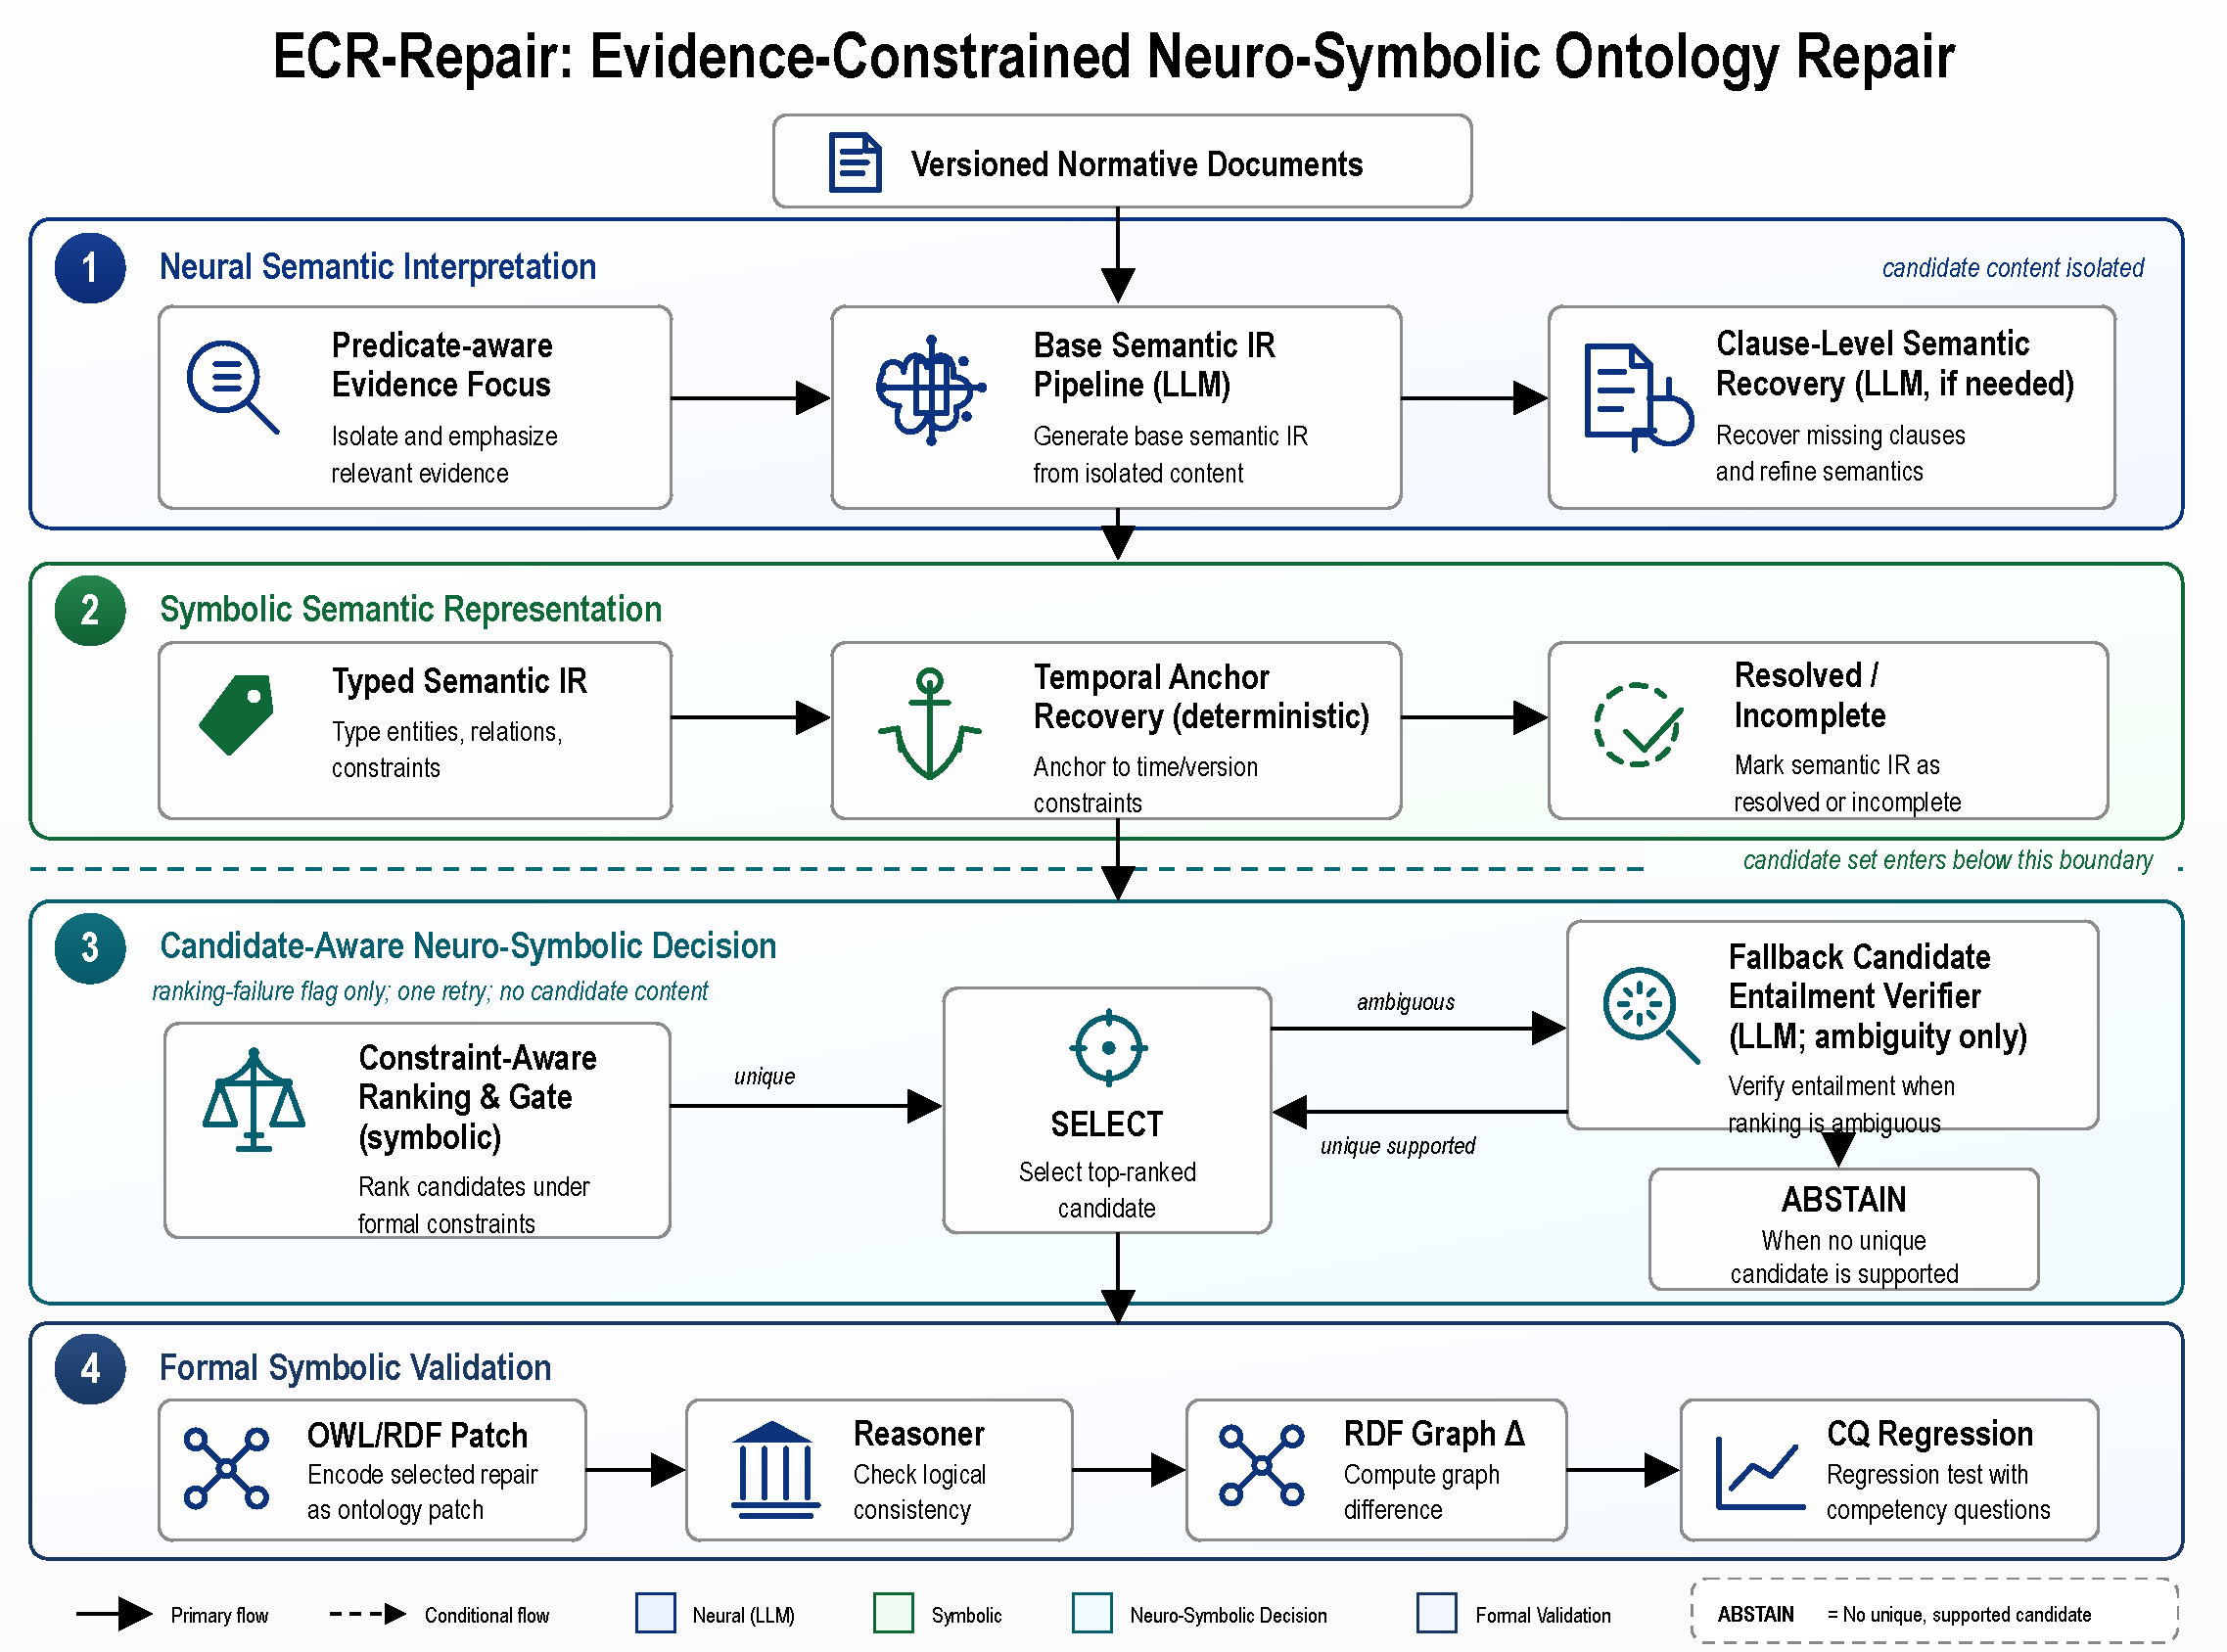
\includegraphics[width=\textwidth]{figures/neurosymbolic_framework.pdf}
    \caption{ECR-Repair 的整体证据约束神经符号架构。Semantic IR 是神经符号接口；候选内容只有在证据解释固定之后才可见。}
    \label{fig:framework}
\end{figure*}

该框架包含五个阶段：
\begin{enumerate}
    \item \textbf{规范证据。} 系统接收版本化规范证据窗口和公开事件元数据。
    \item \textbf{Semantic IR。} LLM 辅助解释模块在不访问候选内容的情况下，将证据转换为类型化语义字段。
    \item \textbf{符号决策。} 确定性评分器基于固定 IR 对候选操作排序，并应用选择性门控。
    \item \textbf{回退验证。} 如果排序无法识别唯一可接受候选，则候选级蕴含验证器独立评估候选。
    \item \textbf{OWL/RDF 验证。} 被选编辑被实体化，随后进行 OWL 一致性检查、RDF 图差分比较和能力问题回归测试。
\end{enumerate}

\subsection{作为神经符号接口的 Semantic IR}

Semantic IR 是语言解释与符号修复之间的核心接口契约。它不是 prompt engineering 的新名称，也不是自由文本理由或候选答案，而是在任何候选内容可见之前，对证据中关于目标断言语义内容的类型化表示。

对每个修复事件，Semantic IR 记录：
\begin{itemize}
    \item \textbf{Entity}：断言涉及的 subject、object、版本、标准、条件或其他规范实体；
    \item \textbf{Relation}：相关谓词、规则关系、例外关系、版本关系或作用域关系；
    \item \textbf{Temporal information}：当前版本、被取代版本、生效日期、发布日期、引用日期或未解析时间锚点；
    \item \textbf{Scope}：被限定语、例外、条件或跨句修饰语支配的陈述或陈述集合；
    \item \textbf{Constraint}：类型限制、规则优先级、否定、数值/日期约束和可接受性条件；
    \item \textbf{Evidence}：支持抽取字段的显式文本片段或文档片段。
\end{itemize}

该表示具有类型特异性。Temporal-Version 事件编码当前、被取代、生效、发布和引用角色；General Rule-Exception 事件编码一般规则、例外触发、例外结果和优先级；Cross-Sentence Scope 事件编码被限定陈述、限定语、作用域目标和附着关系。如果必要字段无法被证据支持，则 IR 被标记为不完整，系统弃权或执行一次候选盲恢复。

该结构体现了方法的神经符号性质：神经组件解释复杂规范语言，符号组件接收可检查、可约束并可映射到形式本体编辑的类型化对象。

\subsection{候选内容隔离}

候选内容隔离是核心设计约束。在证据解释阶段，模型只看到证据窗口和公开事件元数据，而看不到候选值、候选操作、候选标识符、候选分数或私有 oracle。候选信息只有在 Semantic IR 生成并归一化之后才进入系统。

这避免了一条重要泄漏路径：如果提示同时包含证据和候选文本，LLM 可能选择措辞最像证据的候选，而不构造独立语义表示。这类系统可能在有限选择基准上显得准确，却无法提供稳定的证据到本体接口。ECR-Repair 首先固定语义解释：
\[
\text{Evidence}
\rightarrow
\text{Semantic IR}
\rightarrow
\text{Candidate Ranking}.
\]
只有无内容的失败信号可以向后流动。对于 General Rule-Exception 和 Cross-Sentence Scope 事件，如果候选排序未能产生唯一可接受候选，语义恢复模块最多接收布尔标志 \texttt{ranking\_failed=true} 并执行一次额外候选盲恢复。它不会接收领先候选、分数、候选值或任何候选派生语义。

\subsection{符号决策与约束评分}

Semantic IR 固定后，ECR-Repair 暴露有限候选集，并根据证据约束表示对每个候选评分。该决策层是符号化的，因为它使用类型化字段、确定性约束和显式门控条件，而不是自由生成。

为便于说明，决策目标可概括为语义匹配加约束满足再减去冲突。在本文实验实现中，词汇-约束评分组件为：
\[
\begin{aligned}
s(c_i)=&0.30s_f+0.26s_t+0.20\max(s_c,s_n)\\
&+0.12s_n+0.08s_c+0.04s_e+b_{\mathrm{sem}}-p_{\mathrm{neg}} .
\end{aligned}
\]
$s_f$、$s_t$、$s_c$、$s_n$ 和 $s_e$ 分别度量与 Semantic IR 的来源族、词汇、代码、数值和精确值一致性。$b_{\mathrm{sem}}$ 奖励版本关系下的 current、integrated 或 superseded 标记，$p_{\mathrm{neg}}$ 惩罚 obsolete、absent、negated 或 reversed 标记。这些权重是 pilot implementation 中固定的启发式设计选择，不是在最终基准上拟合得到的参数；其相对顺序反映了来源族和词汇一致性优先于精确值匹配和小幅语义 bonus 的设计取向。类型特异的约束重排序进一步检查角色、值、方向、例外优先级和作用域附着约束。实验使用冻结门控：默认最低分数为 0.30，General Rule-Exception 和 Cross-Sentence Scope 阈值为 0.24，最小 margin 为 0.00，Temporal-Version 事件允许在时间门控下接受唯一且不矛盾的 top candidate。

门控只在候选唯一且可接受时接受排序结果。候选可能因 Semantic IR 不完整、分数低于阈值、与另一候选在相关约束下并列，或检测到显式冲突而被拒绝。该门控是选择性的：弃权是有效输出，并优先于不受支持的本体编辑。

\subsection{回退验证}

回退验证器只在符号排序仍有歧义时调用。不同于初始 Semantic IR 阶段，验证器是候选感知的。但它独立评估每个候选，而不是在一个提示中要求模型比较所有候选。对于每个候选，验证器判断该候选操作相对于固定证据和 Semantic IR 是 \texttt{supported}、\texttt{contradicted}、\texttt{unrelated} 还是 \texttt{underspecified}。

只有当恰好一个候选以足够置信度被支持时，候选才能继续。多个候选被支持、无候选被支持、低置信度、矛盾或证据不足都会导致 \textsc{Abstain}。这保留了职责分离：验证器可以解决残余语义歧义，但不替代符号门控或形式闭包。

\subsection{形式验证}

最终阶段在图式知识表示、RDF 验证和 OWL 推理实践下验证被选修复是否为合法 OWL/RDF 操作 \cite{hogan2021knowledgegraphs,pareti2021shaclreview,heist2021caligraph}。每个候选具有声明编辑集：
\[
\Delta_{c_i}=(\Delta^-_{c_i},\Delta^+_{c_i}),
\]
其中 $\Delta^-_{c_i}$ 包含目标删除，$\Delta^+_{c_i}$ 包含目标新增。将候选应用到 $O$ 得到修复后本体 $O'$。ECR-Repair 只有在以下形式验证全部通过时才接受补丁：
\begin{itemize}
    \item \textbf{OWL consistency}：对修复后本体进行物化，并在配置推理机下检查逻辑一致性；
    \item \textbf{RDF graph delta}：实际图差分与候选声明的新增和删除一致，且没有未声明副作用；
    \item \textbf{CQ regression}：冻结的能力问题或修复回归检查在补丁后仍返回预期结果。
\end{itemize}

这些检查提供形式安全性，但不能替代语义选择。语义错误候选仍可能逻辑一致。因此，ECR-Repair 将形式验证视为语义修复的必要但非充分条件。

\section{实验}

\subsection{数据集}

据我们所知，目前没有现成基准能够直接评估版本化规范文档语义漂移下的证据相对本体修复。现有本体修复、知识图谱补全或文档 grounding 问答资源没有同时提供演化规范证据、局部本体断言、可执行 OWL/RDF 修复候选和形式闭包检查。因此，本文构建了一个基于 RFC 的有限候选基准。每个事件包含一个局部本体断言、当前规范证据、语义类型和三个可执行修复候选。候选集包含一个人工审查的证据支持修复，以及两个可执行但语义错误的干扰项，例如保留过时版本、反转 supersession 关系、错配例外条件，或将作用域限定语附着到错误陈述。

一个具体 Temporal-Version 事件可包含：Candidate A 删除 \texttt{(:s :currentSpec :X)} 并添加 \texttt{(:s :currentSpec :Y)}；Candidate B 保留或重申 \texttt{(:s :currentSpec :X)}；Candidate C 以 \texttt{(:X :supersedes :Y)} 反转更新方向。三者都是可执行图编辑，但当证据表明 $Y$ 更新 $X$ 并支配当前要求时，只有 Candidate A 被支持。Table~\ref{tab:dataset} 总结了该基准。

\begin{table}[t]
\centering
\caption{数据集概况}
\label{tab:dataset}
\begin{tabular}{lr}
\toprule
Item & Value \\
\midrule
Events & 264 \\
Runs & 1320 \\
Types & 3 \\
Candidates/event & 3 \\
\bottomrule
\end{tabular}
\end{table}

三类事件对应框架处理的主要语义漂移模式：Temporal-Version、General Rule-Exception 和 Cross-Sentence Scope。评估单位是局部修复事件，而不是完整本体规模。实验因此衡量的是，在潜在漂移事件及其证据窗口已给定后，方法能否选择并验证正确的局部 OWL/RDF 补丁。

\subsection{比较方法}

我们比较三种方法。\textbf{Direct LLM} 接收证据和候选内容，并直接从候选中选择。它代表自然提示基线，但不执行候选内容隔离或形式闭包。\textbf{Base Semantic IR} 使用证据 grounding 的 Semantic IR 和符号修复逻辑，但不包含完整 ECR-Repair 的恢复与回退验证设计。\textbf{ECR-Repair} 使用 Section IV 描述的完整流水线，包括候选内容隔离的 Semantic IR、约束感知符号决策、回退验证和 OWL/RDF 验证。

这些基线的目标不是比较 token 成本或延迟。Direct LLM 与 ECR-Repair 具有不同调用结构，因为 ECR-Repair 分离了语义解释、排序、验证和形式闭包。该比较关注显式神经符号结构是否能相较直接候选选择和基础 Semantic IR 流水线提高修复可靠性。

\subsection{评价指标}

闭包准确率是指方法选择证据支持候选，并且对于修复流水线而言，其对应 OWL/RDF 补丁通过形式验证的运行比例。严格成功率是事件级成功率：只有当方法在该事件的重复运行中全部成功时，该事件才算严格成功。Direct LLM 不报告严格成功率，因为该基线直接选择候选且不执行完整形式闭包流水线；因此 Table~\ref{tab:main_result} 使用闭包准确率作为共同比较指标。

\subsection{主结果}

Table~\ref{tab:main_result} 报告主比较。ECR-Repair 达到 99.62\% 闭包准确率和 99.24\% 严格成功率，显著优于两个基线。Direct LLM 在直接暴露候选的条件下达到 93.48\%，说明任务对语言模型并非不可行。然而，其剩余错误说明有必要分离证据解释与候选选择，并对最终修复进行形式验证。Base Semantic IR 达到 77.42\% 闭包准确率和 73.86\% 严格成功率，表明结构化证据解释本身仍不充分；候选内容隔离必须与约束感知排序、选择性门控和回退验证结合。

\begin{table}[t]
\centering
\caption{会议基准上的主结果}
\label{tab:main_result}
\begin{tabular}{lcc}
\toprule
Method & Closure Accuracy & Strict Success \\
\midrule
Direct LLM & 93.48\% & -- \\
Base Semantic IR & 77.42\% & 73.86\% \\
ECR-Repair & 99.62\% & 99.24\% \\
\bottomrule
\end{tabular}
\end{table}

\subsection{错误分析}

剩余失败表现为弃权，而不是输出不受支持的补丁。一个代表性失败是 General Rule-Exception 事件：Semantic IR 能识别相关规则和例外，但验证器无法在固定门控下隔离唯一被证据支持的候选。类似边界情况也出现在限定语可能附着到多个相邻陈述时。因此，残余风险是可执行候选之间的例外或作用域解析不足，而不是 OWL 物化失败。

\section{讨论}

会议版评估的是在潜在事件、证据窗口和有限候选集已给定后的修复决策质量；全语料漂移发现、证据检索和候选生成属于后续期刊扩展。形式验证是必要但非充分条件：OWL 一致性、RDF 图差分检查和 CQ 回归能够发现意外形式影响，但不能单独决定语义支持。因此，ECR-Repair 将 LLM 限制在证据解释和残余蕴含判断中，而不是将其作为无约束本体编辑器。当前基准使用人工审查候选；后续公开数据集发布将包含系统化标注者一致性研究，以进一步增强基准可靠性。

\section{结论}

本文提出 ECR-Repair，一种面向版本化规范文档语义漂移的证据约束神经符号本体修复框架。它使用 Semantic IR 作为神经符号接口，在语义解释期间隔离候选内容，通过符号约束排序候选，选择性验证歧义，并通过 OWL 一致性、RDF 图差分和 CQ 回归验证被选补丁。在 264 个 RFC 修复事件和 1320 次运行上，ECR-Repair 达到 99.62\% 闭包准确率和 99.24\% 严格事件成功率，说明可靠修复需要在证据解释、符号决策、选择性弃权和形式闭包之间进行严格职责分离。

\bibliographystyle{IEEEtran}
\bibliography{refs}

\end{document}
